\subsection*{Overview}

In order to interact with the robot aside of speech, a web-based Graphical User Interface (GUI) has been designed. An HTML5 website\footnote{\texttt{https://github.com/tue-robotics/tue\_mobile\_ui}} is hosted on the robotic platform that offers a GUI to multiple users on different platforms with use of a Robot API\footnote{\texttt{https://github.com/tue-robotics/robot-api}} implemented in Javascript. Figure~\ref{fig:webgui_architecture} shows an overview of how the user can interact with the robot via this interface. 
\begin{figure}[H]
        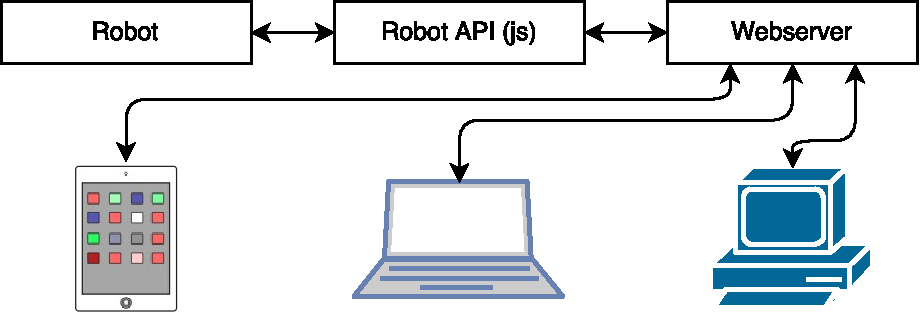
\includegraphics[width = \linewidth]{webgui_architecture}
        \caption{Overview webGUI architecture. The robot's functionalities are exposed with use of the Robot API that is implemented in Javascript. The Webserver that is hosting the GUI connects this Robot API to a graphical user interface that is offered to multiple clients on different platforms.}
        \label{fig:webgui_architecture}
\end{figure}
Figure~\ref{fig:gui_actions} illustrates the GUI and the different commands that can be given to the robot while interacting with the virtual scene.


\begin{figure}[H]
        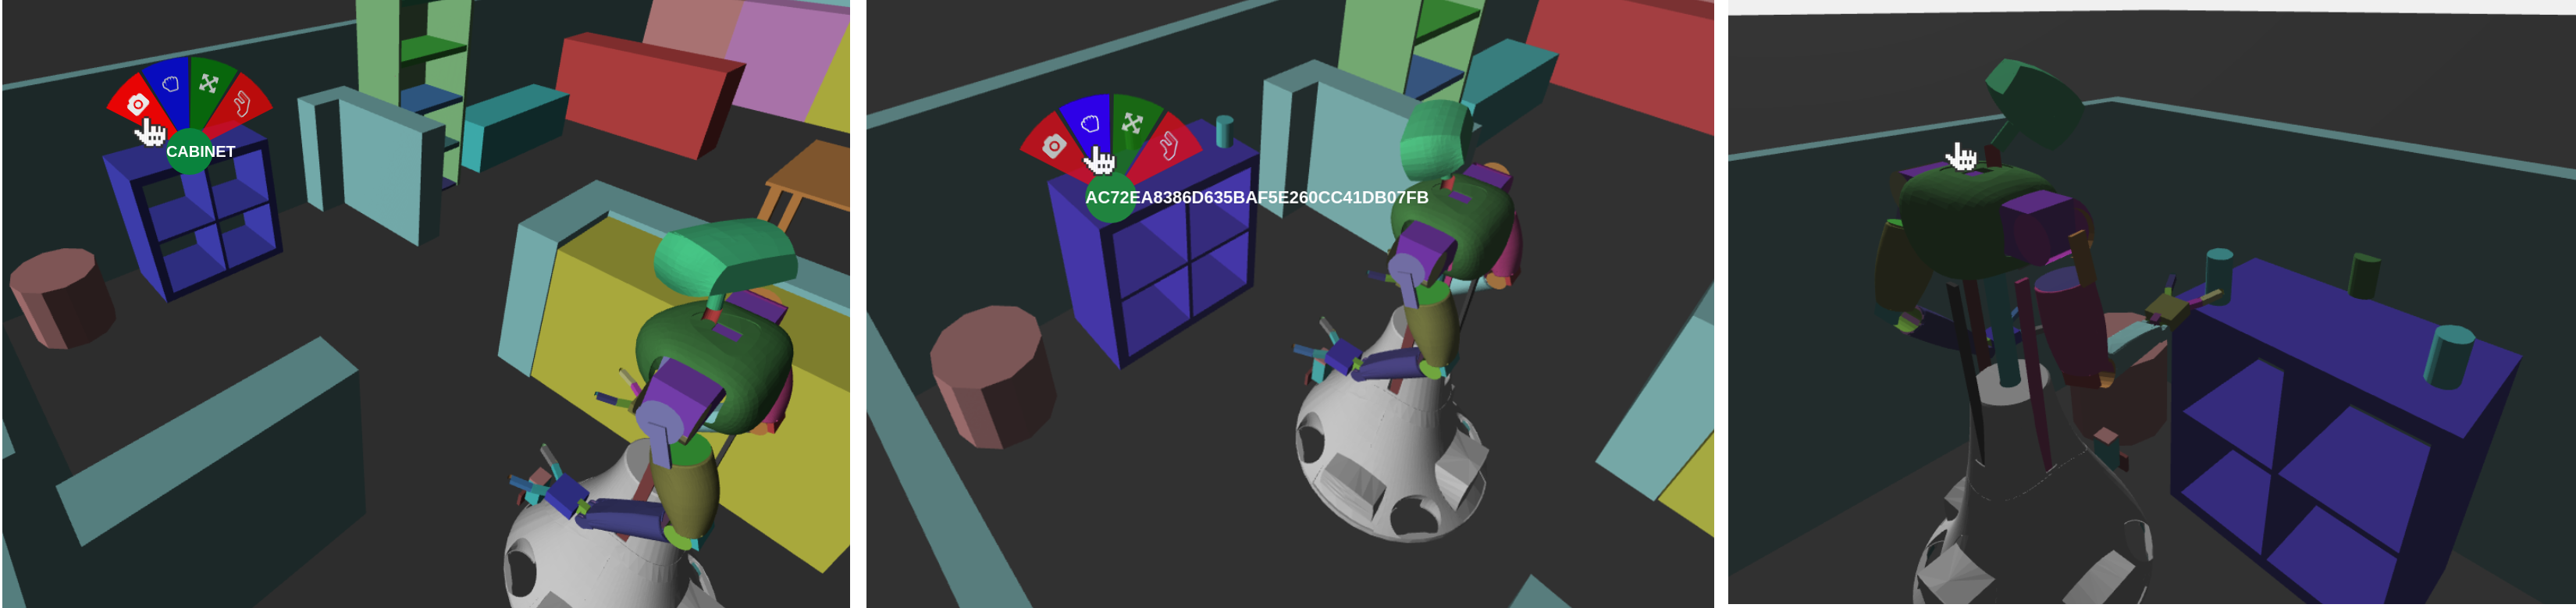
\includegraphics[width = \linewidth]{Figures/gui_actions}
        \caption{Illustration of the 3D scene of the Web GUI. Users can interact with use of the menu that appears when long pressing an object in the scene. On the left figure, the use commands the robot to inspect the selected object, which is the `cabinet'. When the robot has inspected the `cabinet', it has found entities on top of it. The middle and the right figure illustrate a grasp command and the robot's execution of this action.}
        \label{fig:gui_actions}
\end{figure}

These actions are passed via the Robot API to the action server that schedules the actions the robot has to perform. This action server enables various clients to give task commands to the robot. Other clients that make use of this action server are Speech and the Natural Language Console, explained in Section~\ref{sec:nli}.

